\chapter{Five Beginner Entrepreneurial Moves}

This chapter follows a School of Hard Knocks entrepreneurship lesson curated by LazyingArt LLC through Video2Book. The source is not a formal classroom lecture with a board full of equations; it is a walking, conversational talk about what a beginner entrepreneur should know before the abstractions get too clean. We will keep that order. First comes the reason for continuing, then the cash needed to survive, then the five operating moves: sales, accounting, onboarding, content, and networking.

\section{A Trail Walk Instead of a Boardroom}

The speaker begins by changing the setting. He is not trying to make entrepreneurship sound like a solemn ceremony. He says the video will be a trail walk because business, entrepreneurship, and finance content often becomes too serious, when what a beginner often needs is closer to a conversation with a younger self.

That opening is not decoration. It tells us how to read the rest of the lesson. The advice is practical hindsight. It is not a theory of firms, and it is not an audited case study. It is a map of beginner constraints: what holds the founder together, what keeps the bills paid, what gets customers in, what prevents preventable losses, and what allows relationships to compound.

We can summarize the lecture's governing order as follows:
\[
\text{survive personally}
\;\longrightarrow\;
\text{sell commercially}
\;\longrightarrow\;
\text{measure financially}
\;\longrightarrow\;
\text{serve operationally}
\;\longrightarrow\;
\text{grow through attention and relationships}.
\]
The formula is not spoken as mathematics in the video. It is a compact reconstruction of the sequence the speaker follows.

\section{Before the Tips: Why and Cash Runway}

Before giving the numbered tips, the speaker stops on something he calls more important than the tips themselves: finding one's ``why.'' The reason is not sentimental. It is operational. Some days in entrepreneurship feel easy; other days make a founder question the entire project. The ``why'' is the stabilizing term in the system.

Let \(M_t\) denote motivation or commitment at time \(t\). We should not pretend that the speaker gives a psychological model, but the structure of his point can be written cautiously as
\[
M_{t+1}
\approx
M_t
+
Y_t
-
D_t,
\]
where \(Y_t\) is the reinforcing effect of the founder's reason for continuing, and \(D_t\) is discouragement from bad days, negative self-talk, or lack of visible results. The claim is qualitative: without a strong \(Y_t\), repeated discouragement can dominate the process.

\subsection{Question \& Answer}

\paragraph{Question.}
If the business is not yet producing enough results, why keep working so hard?

\paragraph{Answer.}
The speaker's answer is that the founder's ``why'' has to carry some of the load before the market gives clean feedback. The point is not that motivation replaces evidence. It is that early entrepreneurship contains stretches where the evidence is noisy, delayed, or discouraging. During those stretches, a founder needs a reason strong enough to keep showing up while the business is still being built.

The second pre-tip point is more concrete: it is perfectly acceptable to work a job while starting a business. Rent, food, and ordinary living costs do not vanish because a person has begun a company. We can write the beginner survival constraint as
\[
W_t + B_t \geq R_t + F_t + P_t,
\]
where \(W_t\) is job income, \(B_t\) is available business or startup cash, \(R_t\) is rent, \(F_t\) is food, and \(P_t\) represents other personal expenses. In this frame, a job is not the opposite of entrepreneurship. It can be the funding mechanism that lets the founder stay alive long enough to build the business.

There is also a second use for job income:
\[
W_t
=
\text{living support}
+
\text{possible business injection}.
\]
The speaker's practical message is simple: if the business cannot yet fund the founder, outside income can fund both the person and, where possible, the company.

\section{Tip One: Sales as the Golden Rule}

The first numbered tip is given special status. The remaining tips are in no particular order, but this one is the golden rule: know sales. The speaker makes the claim in its most direct commercial form:
\[
\text{no ability to sell}
\;\Longrightarrow\;
\text{no functioning business}.
\]
This is not a statement about personality. It is a statement about exchange. A product or service only becomes a business when customers can be persuaded to buy it.

The speaker then sharpens the point by bringing in churn. Even if customers arrive, some will leave. Customer turnover is real, so the business cannot treat acquisition as a one-time event. Let
\[
C_t = \text{customers at time }t,
\]
\[
N_t = \text{new customers acquired during period }t,
\]
and
\[
L_t = \text{customers lost during period }t.
\]
A minimal customer update rule is
\[
C_{t+1} \approx C_t + N_t - L_t.
\]
This is a standard reconstruction of the speaker's point, not a formula displayed in the video. It captures what he means by saying that if the business is not growing, it is dying. The condition for customer growth is
\[
C_{t+1} > C_t
\quad\Longleftrightarrow\quad
N_t > L_t.
\]
The business must keep finding new ways to market and sell so that acquisition exceeds loss.

\subsection{A Worked Customer Example}

Suppose a small service business begins the month with \(C_t=40\) active customers. During the month it gains \(N_t=8\) new customers, but loses \(L_t=5\) customers through churn or turnover. Then
\[
C_{t+1}
\approx
40 + 8 - 5
=
43.
\]
The business grew by three customers.

If the same business gains only \(N_t=3\) customers while losing \(L_t=5\), then
\[
C_{t+1}
\approx
40 + 3 - 5
=
38.
\]
The business may still be selling, answering calls, and staying busy, but the customer base is shrinking. This is the mathematical skeleton underneath the speaker's warning: growth must be maintained, because churn keeps subtracting.

\section{Training Sales Like an Athlete}

The sales discussion then turns into an anecdote. The speaker recalls advice from his first mentor, Joe Soto, who told him to stop ``playing with his food.'' The phrase means that he was entering sales presentations and demos with potential clients without practicing his pitch.

The analogy is to a professional athlete. An athlete practices, watches film, and corrects performance before the next contest. The speaker says the salesperson should do the same: role play, practice the pitch, rewatch Zoom meetings, listen to how the pitch sounds, and notice how objections or scenarios could have been handled better.

That gives us a feedback loop:
\[
\text{attempt}
\;\longrightarrow\;
\text{record or remember}
\;\longrightarrow\;
\text{review}
\;\longrightarrow\;
\text{adjust}
\;\longrightarrow\;
\text{attempt again}.
\]

\begin{figure}
\centering
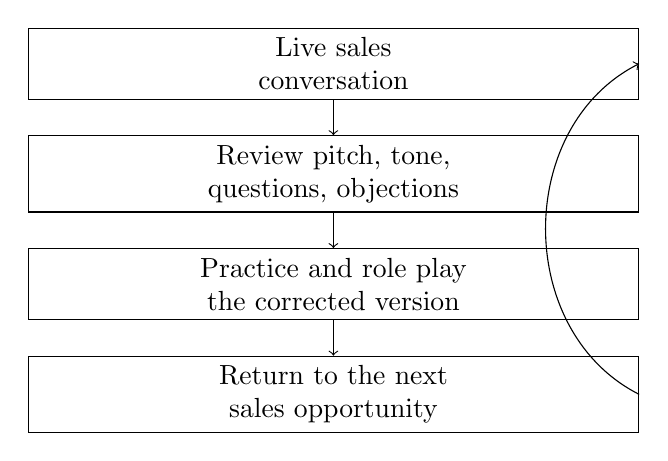
\begin{tikzpicture}[scale=1]
\node[draw, align=center, text width=0.62\linewidth] (a) at (0,0) {Live sales\\conversation};
\node[draw, align=center, text width=0.62\linewidth] (b) at (0,-1.4) {Review pitch, tone,\\questions, objections};
\node[draw, align=center, text width=0.62\linewidth] (c) at (0,-2.8) {Practice and role play\\the corrected version};
\node[draw, align=center, text width=0.62\linewidth] (d) at (0,-4.2) {Return to the next\\sales opportunity};
\draw[->] (a) -- (b);
\draw[->] (b) -- (c);
\draw[->] (c) -- (d);
\draw[->] (d.east) .. controls (2.3,-3.4) and (2.3,-0.8) .. (a.east);
\end{tikzpicture}
\caption{A transcript-derived sales practice loop: the speaker treats sales as a trained skill rather than a one-time performance.}
\end{figure}

The useful distinction is between exposure and training. Merely attending more calls gives exposure. Training requires a loop in which the call is reviewed, the pitch is corrected, and the next attempt is made deliberately.

\section{Accounting and Onboarding: Seeing the Business and Serving the Buyer}

Tip two is accounting. The speaker presents it as advice to his younger self because, by his account, poor financial decisions came from not understanding accounting or how the numbers worked in the business. The central distinction is between the business as imagined and the business as measured:
\[
\text{felt condition of the business}
\neq
\text{measured condition of the business}.
\]
Accounting is the discipline that reduces this gap. It gives the founder a clearer picture of where the business actually stands, and it allows better decisions before the consequences become expensive.

Tip three turns from internal measurement to customer experience. The question is: after someone decides to purchase from the business, what happens next? The sale is not the end of the process. It is the beginning of a new risk interval.

The speaker names two risks. First, buyer's remorse: a customer can regret the decision and attempt a chargeback or cancellation. Second, expectation mismatch: especially in service businesses, unclear communication can create problems later. The onboarding process should therefore teach the customer what to expect, how the relationship works, how communication is handled, and what the next steps are.

We can write the operational function of onboarding as
\[
\text{clear onboarding}
\;\longrightarrow\;
\text{lower remorse}
+
\text{clearer expectations}
+
\text{fewer avoidable conflicts}.
\]
This is not a guarantee. It is a mechanism: the business reduces future disorder by making the post-purchase path explicit.

\begin{figure}
\centering
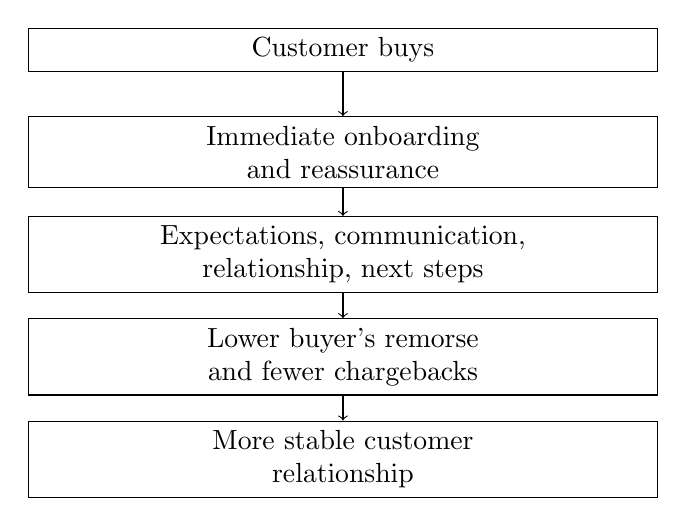
\begin{tikzpicture}[scale=1]
\node[draw, align=center, text width=0.64\linewidth] (a) at (0,0) {Customer buys};
\node[draw, align=center, text width=0.64\linewidth] (b) at (0,-1.3) {Immediate onboarding\\and reassurance};
\node[draw, align=center, text width=0.64\linewidth] (c) at (0,-2.6) {Expectations, communication,\\relationship, next steps};
\node[draw, align=center, text width=0.64\linewidth] (d) at (0,-3.9) {Lower buyer's remorse\\and fewer chargebacks};
\node[draw, align=center, text width=0.64\linewidth] (e) at (0,-5.2) {More stable customer\\relationship};
\draw[->] (a) -- (b);
\draw[->] (b) -- (c);
\draw[->] (c) -- (d);
\draw[->] (d) -- (e);
\end{tikzpicture}
\caption{A transcript-derived onboarding chain. The sale creates the need for an organized post-purchase process.}
\end{figure}

\section{Content, Social Media, and Referral Leverage}

Tip four is investing in content and social media. The speaker's reasoning begins with attention. People spend time on social media, looking at feeds, especially when they are at home or on their phones. A business can use that attention if it shares the right kind of content: useful updates, meaningful progress, and evidence of what the business is doing.

He emphasizes first-degree reach: friends, family, and people one already knows. The transcript phrase is slightly ambiguous, but the mechanism is clear. A beginner does not need a national audience before social media matters. The first useful audience may be the immediate network.

The lecture then gives a concrete anecdote about Austin Smith, described as a digital marketing owner. According to the speaker, Austin held up a stack of cash and offered payment for referrals to business owners who could benefit from his services. The embedded claim is that he gave away \(\$10{,}000\), and later closed probably close to \(\$100{,}000\) worth of business because the video went viral locally.

We should preserve the numbers, but keep them source-conscious:
\[
\text{claimed giveaway} = \$10{,}000,
\qquad
\text{claimed closed business} \approx \$100{,}000.
\]
A rough gross multiple is therefore
\[
\frac{\$100{,}000}{\$10{,}000} \approx 10.
\]
This is not net profit, not verified ROI, and not a universal promise. It is an anecdotal gross comparison. The lesson is the mechanism:
\[
\text{clear referral offer}
+
\text{local attention}
+
\text{credible incentive}
\;\longrightarrow\;
\text{introductions}
\;\longrightarrow\;
\text{closed business}.
\]

\section{Networking by Investing in Other People}

The fifth tip is networking, but the speaker immediately distinguishes his version from the usual weak version. Many people go out, hand out business cards, and try to sell their own products and services. The speaker recommends a different pattern: invest in other people's stories. Ask about their products, their services, and why they do what they do.

The key move is to give free advice or free value. The payoff may not arrive immediately. It may come two months later, when the person remembers the interaction and introduces a useful connection. The speaker calls this planting seeds in other people so that the business can grow through relationships over time.

A compact relationship model is
\[
\text{attention to another person}
+
\text{useful free value}
\;\longrightarrow\;
\text{memory and trust}
\;\longrightarrow\;
\text{future referral}.
\]
The time delay matters. Networking is not only immediate conversion. It is the creation of future paths through which business can move.

The speaker closes this section by naming two books as useful resources for building a better network: \emph{How to Win Friends and Influence People} and \emph{Giftology}. In the logic of the lecture, these are not reading-list ornaments. They point to the same principle: relationships are assets, and they must be handled deliberately.

\section{Summary}

The lecture's form is casual, but its sequence is disciplined. First, a founder needs a reason to continue and enough cash runway to survive. Then the business needs sales, because without buyers there is no business. Sales must be trained, not merely attempted. Accounting corrects the founder's picture of reality. Onboarding protects the customer relationship after purchase. Content and social media use attention as leverage. Networking uses generosity and memory as relationship leverage.

The chapter's working equations are reconstructions, not board work:
\[
W_t + B_t \geq R_t + F_t + P_t,
\]
\[
C_{t+1} \approx C_t + N_t - L_t,
\]
and
\[
N_t > L_t.
\]
Together they say what the speaker says in practical language: keep the founder funded, keep customers coming in faster than they leave, and build systems that make the business more than a burst of effort.